\documentclass{beamer}
%
% Choose how your presentation looks.
%
% For more themes, color themes and font themes, see:
% http://deic.uab.es/~iblanes/beamer_gallery/index_by_theme.html
%

% Colores sacados de http://latexcolor.com/, 
% ponerlos en usercolortheme para cambiar los colores de la presentación
\definecolor{persianred}{rgb}{0.8, 0.2, 0.2}
\definecolor{darkbyzantium}{rgb}{0.36, 0.23, 0.33}
\definecolor{burgundy}{rgb}{0.5, 0.0, 0.13}
\definecolor{deepjunglegreen}{rgb}{0.0, 0.29, 0.29}
\definecolor{darkcoral}{rgb}{0.8, 0.36, 0.27} %este ta weno
\definecolor{darkchestnut}{rgb}{0.6, 0.41, 0.38}
\definecolor{deepcarrotorange}{rgb}{0.91, 0.41, 0.17}
\definecolor{firebrick}{rgb}{0.7, 0.13, 0.13}
\definecolor{pastelred}{rgb}{1.0, 0.41, 0.38}
\definecolor{tyrianpurple}{rgb}{0.4, 0.01, 0.24}
\definecolor{orangeDeadPhysicitsSociety}{HTML}{f28165}
\definecolor{skymagenta}{rgb}{0.81, 0.44, 0.69}
\definecolor{patriarch}{rgb}{0.5, 0.0, 0.5}
\definecolor{darkgreen}{rgb}{0.09, 0.45, 0.27}

\usepackage{xcolor}
\usepackage{mathtools}
\usepackage{setspace}


\newcommand{\semitransp}[2][35]{\textcolor{fg!#1}{#2}}


\mode<presentation>
{
  \usetheme{Madrid}      % or try Darmstadt, Madrid, Warsaw, ...
  \usecolortheme[named=burgundy]{structure} %aquí se cambia el colore, 
  \usefonttheme{default}  % or try serif, structurebold, ...
  \setbeamertemplate{navigation symbols}{}
  \setbeamertemplate{caption}[numbered]
} 
\setbeamercovered{transparent=30}

\renewcommand{\thefigure}{}


\usepackage[english]{babel}
\usepackage[utf8]{inputenc}
\usepackage[T1]{fontenc}
\usepackage{svg}
\usepackage{graphicx} % figuras
\usepackage{subfigure} % subfiguras

\usepackage{geometry}
\usepackage{amsmath,amssymb}
\usepackage{setspace}
\usepackage{comment}
\usepackage{hyperref}

%la wea código
\usepackage{algorithm}
\usepackage{algpseudocode}
 
\usepackage{minted}
\setminted{frame=lines, bgcolor=red!5, fontsize=\footnotesize, breaklines}

\renewcommand{\inserttotalframenumber}{\pageref{lastslide}}
\usepackage{appendixnumberbeamer} 

\AtBeginSection[]{
  \begin{frame}
  \vfill
  \centering
  \begin{beamercolorbox}[sep=8pt,center,shadow=true,rounded=true]{title}
    \usebeamerfont{title}\insertsectionhead\par%
  \end{beamercolorbox}
  \vfill
  \end{frame}
}


\title[Auxiliar 1]{Auxiliar 1}
\subtitle{Introducción a objetos en C++}
\author[Computación GPU]{Profesora: Nancy Hitschfeld-Kahler \\ Auxiliar: Vicente González \\ \textit{\scriptsize Basado en las diapositivas de Sergio Salinas }}
\institute[DCC - UChile]{CC7515-1 -- Computación en GPU}  
\date{\today}

\usepackage{etoolbox}
\makeatletter
\patchcmd{\beamer@sectionintoc}{\vskip1.5em}{\vskip0.5em}{}{}
\makeatother


\DeclareUnicodeCharacter{2212}{-}



\begin{document}

\begin{frame}
  \titlepage
\end{frame}

\begin{frame}{ToC}
    \tableofcontents
\end{frame}

\section{Introducción a C++}

\begin{frame}{Introducción a C++}
    \begin{itemize}
        \item Desarrollado por Bjarne Stroustrup en 1983 como una extensión del lenguaje C.
        \item Lenguaje de bajo nivel con control de memoria necesarias para aprovechar la arquitectura de la GPU.
        \item Se recomienda usar el estándar de C++ moderno (C++ 11 en adelante).
    \end{itemize}
\end{frame}

\begin{frame}[fragile]{Hello world}

\begin{minted}[label=hello.cpp]{cpp}
#include <iostream>

int main() {
    std::cout << "Hello, world!" << std::endl;
    return 0;
}

//g++ hello.cpp -o hello
\end{minted}

\end{frame}

\section{Actividad}

\begin{frame}{CPPokemon}

   \begin{itemize}
    \item Crear un pequeño proyecto
    \item Ejecutables y librerias 
    \item Aprender a hacer clases en C++
    \begin{itemize}
        \item Pokemon
        \item Movimientos
        \item Tipos
    \end{itemize}
    \item Uso de CMake y Google Test
    \item Tips del auxiliar para trabajar más cómodamente :D
   \end{itemize}
\end{frame}

\begin{frame}{Proyecto}
    Vamos a crear un proyecto ``típico'' de C++, con las siguientes carpetas:
   \begin{itemize}
       \item \texttt{src}: Donde van todos los archivos .cpp y .h para compilar el proyecto.
       \item \texttt{include}: Reservado para headers ``públicos'' cuando se hacen librerías o usan.
       \item \texttt{external}: Dependencias del proyecto.
       \item \texttt{test}: Donde dejar los tests del proyecto.
       \item \texttt{build}: Donde van a ir nuestros ejecutables y cositas de CMake.
   \end{itemize}
    Clone la repo \url{https://github.com/Seivier/CPPokemon.git}
\end{frame}

\section{Clases en C++}
\begin{frame}{Introducción a Clase en C++}
\begin{itemize}
\item En C++, un objeto es una instancia de una clase.
\item Una clase es una estructura de datos que define un conjunto de atributos y métodos que operan sobre esos atributos.
\item Los objetos se pueden crear dinámicamente en tiempo de ejecución usando punteros y el operador \texttt{new}.
%\item La notación de punto (\texttt{.}) se utiliza para acceder a los atributos y métodos de un objeto.
\item Los objetos se eliminan usando el operador \texttt{delete} para liberar la memoria asignada a ellos.
\item Se pueden usar tanto \texttt{class} como \texttt{struct}
\end{itemize}
\end{frame}

%Declaración de una clase
%

\subsection{Clases abstractas}

\begin{frame}[fragile]{Declaración}
\begin{minted}[label=pkm.h]{cpp}
struct Pokemon {
  virtual void speak() const = 0;
  virtual const std::string& name() const = 0;
  virtual int hp() const = 0;
  virtual int maxHp() const = 0;
  virtual const Type& type() const = 0;
};
\end{minted}
\begin{center}
    Una \textit{interface} en C++ !!!
\end{center}
\end{frame}

\subsection{Creación de un objeto}

\begin{frame}[fragile]{Declaración}
\begin{itemize}
    \item Cree las clases \texttt{APokemon}, \texttt{AMovement} y \texttt{AType} donde encapsule el funcionamiento común
    \item Para \texttt{APokemon} puede crear variables privadas para la vida y el tipo.
    \item Para \texttt{AMovement} puede crear variables privadas para el poder, el tipo y la precisión del ataque.
    \item Para \texttt{AType} puede establecer el comportamiento por defecto de las funciones.
\end{itemize}
\end{frame}


\begin{frame}[fragile]{Declaración}
\begin{minted}[label=Ejemplo]{cpp}
class APokemon {
public:
  // ...
  int hp() const override;
private:
  // ...
  int _hp; // o mHp;
};
\end{minted}
\begin{center}
    Recuerde que la declaración va en un .h y la implementación en un .cpp
\end{center}
\end{frame}

\section{Constructores}

\begin{frame}[fragile]{Tipos de constructores y destructores}

\begin{minted}{cpp}
    // Constructor por defecto
    Rectangulo(): ancho(0), alto(0) {}

    // Constructor con parámetros
    Rectangulo(double ancho, double alto) {
        this->ancho = ancho; 
        this->alto = alto; }
        
    // Constructor copia
    Rectangulo(const Rectangulo& r) {
        this->ancho = r.ancho; 
        this->alto = r.alto; }
        
    // Destructor
    ~Rectangulo() {
        std::cout << "Se ha destruido un rectangulo." << std::endl;
    }    
\end{minted}
\end{frame}

\begin{frame}{Tipos de constructores y destructores}
\begin{itemize}
    \item Cree constructores para sus clases, donde inicialize cada variable
    \item Aseguresé de crear todo lo necesario en el constructor
    \item Debe hacerse cargo de la memoria pedida en el destructor
\end{itemize}
\begin{center}
    \alert{IMPORTANTE!}

    Usted no puede usar una clase abstracta como miembro de la clase, un lugar de eso deber usar un puntero
\end{center}
\end{frame}

\section{Biblioteca estándar de C++}

\begin{frame}[fragile]{Biblioteca estándar de C++}
Conjunto de funciones, objetos y clases que proporcionan una amplia variedad de características y funcionalidades para el lenguaje C++. Por ejemplo:

\begin{itemize}
\item Entrada/salida: operaciones de entrada y salida, como leer o escribir en archivos o en la consola.
\item Contenedores: estructuras de datos para almacenar y manipular colecciones de objetos, como vectores, listas, mapas, etc.
\item Algoritmos: funciones para realizar operaciones comunes en contenedores, como ordenar, buscar, mezclar, etc.
\item Tipos de datos: tipos de datos comunes, como cadenas de caracteres, booleanos, números, etc.
\item Funciones matemáticas: funciones matemáticas comunes, como seno, coseno, exponencial, etc.
\end{itemize}

La Biblioteca estándar de C++ está disponible en cualquier compilador que cumpla con el estándar de C++. Para usarla, se debe incluir el archivo de cabecera correspondiente.
\end{frame}

\begin{frame}{Bibliotecas de la librería estandar}

\begin{itemize}
\item \texttt{<iostream>}: para entrada/salida de consola
\item \texttt{<vector>}: para el uso de vectores dinámicos
\item \texttt{<string>}: para el uso de cadenas de texto
\item \texttt{<algorithm>}: para el uso de algoritmos de ordenación, búsqueda, etc.
\item \texttt{<unordered\_map>} y \texttt{<map>}: para el uso de mapas y diccionarios
\item \texttt{<set>}: para el uso de conjuntos
\item \texttt{<cmath>}: para el uso de funciones matemáticas como \texttt{sqrt()}, \texttt{cos()}, \texttt{sin()}, etc.
\item \texttt{<chrono>}: para el uso de medidas de tiempo
\item \texttt{<memory>}: para el uso de puntero inteligentes
\item etc
\end{itemize}

Más en \url{https://en.cppreference.com/w/cpp/standard_library}

\end{frame}

\begin{frame}{Memory}

\begin{itemize}
\item Existen 3 tipos de punteros ``inteligentes'' en la STL
\item Funcionan como puntero normales desde afuera
\item El uso correcto de estos garantiza el despreocuparse por el manejo de memoria
\item \texttt{std::shared\_ptr<T>}: Permite crear un puntero compartido, va contando las referencias y autodestruye cuando el contador llega a 0
\item \texttt{std::unique\_ptr<T>}: Permite crear un puntero único, el cual no permite compartir la información que contiene con otros punteros
\item \texttt{std::weak\_ptr<T>}: Permite crear un puntero débil, se comporta de manera similar a un puntero clásico y sirve para referencia cíclicas
\end{itemize}

\end{frame}

\begin{frame}[fragile]{Memory}
\begin{center}
    Reemplace sus punteros clásicos por \texttt{std::unique\_ptr<T>}, puede usar \texttt{std::make\_unique<T>} para crear uno
\end{center}

\begin{minted}[label=Ejemplo]{cpp}
class C {
public:
    int x, y, z;
    C(int x, int y, int z);

}

int main() {
    std::unique_ptr<C> p;
    p = std::make_unique<C>(10, 20, 30); // llama al constructor 
    std::cout << p->x << std::endl; // "10"
}
\end{minted}
\end{frame}

\begin{frame}[fragile]{String}

\begin{itemize}
\item Permite manejar strings de manera cómoda
\item Funciona como cualquier string de otro lenguaje tipado
\end{itemize}
\end{frame}

\begin{frame}[fragile]{String}
Añada la siguiente función a \texttt{Pokemon}
\begin{minted}[label=pkm.h]{cpp}
struct Pokemon {
    // ...
    virtual const std::string& name() const = 0;
}
\end{minted}

E implementela en la clase abstracta

\end{frame}

\begin{frame}[fragile]{Vector}

\begin{itemize}
\item Los vectores de la STL son arreglos típicos de otros lenguajes
\item Permiten manipular arreglos de tamaño dínamico alojados en el heap
\item Usando esto y los punteros inteligentes puede evitar tratar con \texttt{new} y \texttt{delete} casi en su totalidad
\end{itemize}
\end{frame}

\begin{frame}[fragile]{Vector}
Añada a \texttt{APokemon} un arreglo de movimientos \texttt{Movement}

\end{frame}
\section{Overloading}

\begin{frame}[fragile]{Overloading de operadores}

El \textbf{overloading de operadores} es una funcionalidad en C++ que permite a los desarrolladores definir una función que se comporta como un operador. Por ejemplo, para sumar dos números complejos, podemos sobrecargar el operador \texttt{+} de la siguiente manera:

\begin{minted}{c++}
class Complejo {
public:
    Complejo operator+(const Complejo& c) const {
        return Complejo(real + c.real, imag + c.imag);
    }
private:
    double real;
    double imag;
};
\end{minted}

En este caso, estamos sobrecargando el operador \texttt{+} para que sume dos números complejos. El operador se define dentro de la clase \texttt{Complejo} y se utiliza el operador \texttt{+} para definir la función.
\end{frame}
\begin{frame}[fragile]{Overloading de operadores}
Añada la siguientes funciones a \texttt{Pokemon} en \texttt{util/pkm.h}
\begin{minted}[label=pkm.h]{cpp}
struct Pokemon {
    // ...
    virtual Movement& operator[](const std::size_t idx) const = 0;
}
std::ostream& operator<<(std::ostream& os, const Pokemon& pok);
\end{minted}

E implementela en la clase abstracta
\end{frame}

\section{Compilación}

\begin{frame}{Compilación}
    Creemos unas clases concretas para poder compilar el proyecto
    \begin{itemize}
        \item Los tipos Normal, Rock y Fighting.
        \item Los siguientes Pokémon:
        \begin{itemize}
            \item Bidoof de tipo Normal con 60 de vida
            \item Mankey de tipo Fighting con 100 de vida
        \end{itemize}
        \item Los siguientes Movimientos:
        \begin{itemize}
            \item Tackle de tipo Normal con 40 de poder y 100 de precisión
            \item CrossChop de tipo Fighting con 100 de poder y 80 de precisión
            \item Rollout de tipo Rock con 30 de poder y 90 de precisión
        \end{itemize}
    \end{itemize}
\end{frame}

\begin{frame}[fragile]{Compilación}
\begin{minted}[label=Makefile]{make}
INC=include/
SRC=main.cpp pokemon.cpp movement.cpp
BUILD=build/

.PHONY: build clean

build:
    mkdir -p build/
    $(CC) $(LDFLAGS) $(SRC) -I$(INC) -o $(BUILD)main

clean:
    rm -rf build
\end{minted}
\end{frame}


\begin{frame}[fragile]{CMake o Makefile?}
    \begin{itemize}
        \item CMake
        \begin{itemize}
            \item Estándar moderno de C++
            \item Complejo y estructurado
            \item Multiplataforma
            \item Relativamente intuitivo
            \item Basado en macros y funciones
        \end{itemize}
        \item Makefile
        \begin{itemize}
            \item Pensado con \emph{build tool} de Linux
            \item Sencillo y directo
            \item Basado en reglas
            \item Ideal para automatizar comandos
        \end{itemize}
    \end{itemize}
\end{frame}

\begin{frame}[fragile]{Compilación}
\begin{minted}[label=Cmake en bash]{bash}
$ cmake -S . -B build 
    # S es para el codigo fuente
    # B es donde dejar los archivos generados

$ cmake --build build 
    # build construye en ejectable o libreria

$ ./build/src/CPPokemonRun
    # con esto se ejecuta la aplicación
\end{minted}
\end{frame}
%
% \begin{frame}[fragile]
% \frametitle{Ejemplo de Overloading}
%
% \begin{columns}
%     \begin{column}{0.62\textwidth}
%         \begin{minted}[label=Complejo.h]{c++}
% class Complejo {
% private:
%     double real, imag;
% public:
%     Complejo(double r = 0, double i = 0) : real(r), imag(i) {}
%     Complejo operator+(Complejo const &obj) {
%         Complejo res;
%         res.real = real + obj.real;
%         res.imag = imag + obj.imag;
%         return res;
%     }
%     void imprimir() {
%         std::cout << real << " + " << imag << "i" << std::endl;
%     }
% };
%         \end{minted}
%     \end{column}
%
%     \begin{column}{0.38\textwidth}
%         \begin{minted}[label=main.cpp]{c++}
% int main() {
%     Complejo a(3.0, 4.0);
%     Complejo b(2.0, 3.0);
%     Complejo c = a + b;
%     c.imprimir();
%     return 0;
% }
%         \end{minted}
%     \end{column}
% \end{columns}
%
% \end{frame}


% \begin{frame}[fragile]{Ejemplo de friend class en C++}
% \begin{columns}
%   \begin{column}{0.5\textwidth}
%   %\vspace{-2cm}
% \begin{minted}[fontsize=\footnotesize, ]{cpp}
% class Complejo {
% private:
%     ...
% public:
%     friend std::ostream& operator<<(std::ostream& out, const Complejo& c);
%     friend std::istream& operator>>(std::istream& in, Complejo& c);
% };
%
% std::ostream& operator<<(std::ostream& out, const Complejo& c) {
%     out << c.real << " + " << c.imag << "i";
%     return out;
% }
%     \end{minted}
%   \end{column}
%   \begin{column}{0.5\textwidth}
%     \begin{minted}[fontsize=\footnotesize, frame=lines, breaklines]{cpp}
% std::istream& operator>>(std::istream& in, Complejo& c) {
%     cin >> c.real;
%     cin >> c.imag;
%     return in;
% }
%
% int main() {
%     Complejo c1(2, 3), c2;
%     std::cout << "c1 = " << c1 << std::endl;
%     std::cout << "Ingrese un número complejo: ";
%     std::cin >> c2;
%     std::cout << "c2 = " << c2 << std::endl;
%     return 0;
% }
%     \end{minted}
%   \end{column}
% \end{columns}
%
% \end{frame}
%
%
% \section{Templates}
%
% \begin{frame}[fragile]{Templates en C++}
%
% Los templates son una característica de C++ que permiten escribir funciones y clases genéricas que pueden trabajar con diferentes tipos de datos sin tener que escribir múltiples versiones para cada tipo de dato.
%
% \begin{minted}[label={maximo.hpp}]{c++}
% template <typename T>
% T maximo(T a, T b) {
% return a > b ? a : b;
% }
%
% int a = 5, b = 10;
% maximo(a, b);
%
% double c = 3.14, d = 2.71;
% maximo(c, d);
% std::string s1 = "hola", s2 = "mundo";
% maximo(s1, s2)
% }
% \end{minted}
%
% \end{frame}
%
% \begin{frame}[fragile]{Templates}
% \begin{columns}
% \column{0.4\textwidth}
% \begin{minted}[label=Declaración]{c++}
% template <typename T>
% class Rectangulo {
% private:
%     T ancho;
%     T alto;
% public:
% Rectangulo(T ancho, T alto)
% {
%     this->ancho = ancho;
%     this->alto = alto;
% }
%
% T calcular_area() {
%     return ancho * alto;
% }
% };
% \end{minted}
%
% \column{0.6\textwidth}
% \begin{minted}[label=Llamada]{c++}
% int main(){
%     Rectangulo<int> rect1(4, 5);
%     rect1.calcular_area();
%     Rectangulo<float> rect2(2.5, 3.5);
%     rect2.calcular_area();
%     return 0;
% }
% \end{minted}
% \end{columns}
% \end{frame}
%
%
% \section{Biblioteca estándar de C++}
%
% \begin{frame}[fragile]{Biblioteca estándar de C++}
% Conjunto de funciones, objetos y clases que proporcionan una amplia variedad de características y funcionalidades para el lenguaje C++. Por ejemplo:
%
% \begin{itemize}
% \item Entrada/salida: operaciones de entrada y salida, como leer o escribir en archivos o en la consola.
% \item Contenedores: estructuras de datos para almacenar y manipular colecciones de objetos, como vectores, listas, mapas, etc.
% \item Algoritmos: funciones para realizar operaciones comunes en contenedores, como ordenar, buscar, mezclar, etc.
% \item Tipos de datos: tipos de datos comunes, como cadenas de caracteres, booleanos, números, etc.
% \item Funciones matemáticas: funciones matemáticas comunes, como seno, coseno, exponencial, etc.
% \end{itemize}
%
% La Biblioteca estándar de C++ está disponible en cualquier compilador que cumpla con el estándar de C++. Para usarla, se debe incluir el archivo de cabecera correspondiente.
% \end{frame}
%
% \begin{frame}{Bibliotecas de la librería estandar}
%
% \begin{itemize}
% \item \texttt{<iostream>}: para entrada/salida de consola
% \item \texttt{<vector>}: para el uso de vectores dinámicos
% \item \texttt{<string>}: para el uso de cadenas de texto
% \item \texttt{<algorithm>}: para el uso de algoritmos de ordenación, búsqueda, etc.
% \item \texttt{<unordered\_map>} y \texttt{<map>}: para el uso de mapas y diccionarios
% \item \texttt{<set>}: para el uso de conjuntos
% \item \texttt{<cmath>}: para el uso de funciones matemáticas como \texttt{sqrt()}, \texttt{cos()}, \texttt{sin()}, etc.
% \item \texttt{<chrono>}: para el uso de medidas de tiempo
% \item \texttt{<thread>}: para el uso de hilos de ejecución
% \item etc
% \end{itemize}
%
% Más en \url{https://en.cppreference.com/w/cpp/standard_library}
%
% \end{frame}
%
% \begin{frame}[fragile]
%   \frametitle{Ejemplo de string y métodos}
%   \begin{columns}
%     \begin{column}{0.3\textwidth}
%       \begin{itemize}
%         \item \texttt{size()}
%         \item \texttt{length()}
%         \item \texttt{empty()}
%         \item \texttt{clear()}
%         \item \texttt{substr()}
%         \item \texttt{find()}
%         \item \texttt{replace()}
%       \end{itemize}
%     \end{column}
%     \begin{column}{0.7\textwidth}
%       \begin{minted}[label=string\_example.cpp]{cpp}
% #include <iostream>
% #include <string>
% using namespace std;
%
% int main() {
%   string str = "Hello, world!";
%   cout<<"\n str = "<<str;
%   cout<<"\n size = "<<str.size();
%   cout<<"\n substring = "<<str.substr(0, 5);
%   int pos = str.find("mundo"); //pos = 5
%   if(str.empty()) 
%   cout << "La cadena esta vacia";
%   else cout<<"La cadena tiene"<<str.length()
%   <<" caracteres";
%
%   return 0;
% }
%       \end{minted}
%     \end{column}
%   \end{columns}
% \end{frame}
%
% \begin{frame}[fragile]{Métodos de vector en C++}
% \begin{columns}
% \begin{column}{0.3\textwidth}
%     \begin{itemize}
% \item \texttt{size()}
% \item \texttt{push\_back()}
% \item \texttt{pop\_back()}
% \item \texttt{insert()}
% \item \texttt{erase()}
% \item \texttt{clear()}
% \item \texttt{reserve()}
% \item \texttt{empty()}
%     \end{itemize}
% \end{column}
%
%     \begin{column}{0.7\textwidth}
%     \begin{minted}[label=vector\_example.cpp]{cpp}
% #include <iostream>
% #include <vector>
% using namespace std;
%
% int main() {
%     vector<int> v;
%     v.push_back(10);
%     v.push_back(20); //{10, 20}
%     v.pop_back(); //20
%     v.insert(v.begin() + 1, 30); //{10, 30, 20}
%     v.erase(v.begin() + 1); //{10, 20}
%     v.clear();
%     v.reserve(100);
%     if (v.empty())
%         cout << "El vector está vacío" << endl;
%     return 0;
% }
%     \end{minted}
%         \end{column}
% \end{columns}
%
% \end{frame}
%
% \begin{frame}[fragile]{Iteradores en un vector de C++}
%
% \begin{columns}
% \begin{column}{0.5\textwidth}
% Un iterador es un objeto que se utiliza para recorrer una secuencia de elementos en un contenedor, como un vector.
%
% \begin{itemize}
%     \item \texttt{begin()}: devuelve un iterador al primer elemento del vector.
%     \item \texttt{end()}: devuelve un iterador al último elemento del vector.
%     \item \texttt{rbegin()}: devuelve un iterador al último elemento del vector.
%     \item \texttt{rend()}: devuelve un iterador al primer elemento del vector.
% \end{itemize}
%
% \end{column}
%
% \begin{column}{0.5\textwidth}
%
% \begin{minted}[fontsize=\small, frame=lines, label=Ejemplo]{c++}
% #include <iostream>
% #include <vector>
% int main() {
%     std::vector<int> vec = {1, 2, 3, 4, 5};
%     // Recorrer el vector con un iterador
%     for (auto it = vec.begin(); it != vec.end(); ++it) {
%         std::cout << *it << " ";
%     }
%     return 0;
% }
%     \end{minted}
% \end{column}
% \end{columns}
%
% \end{frame}
%
%
% \begin{frame}[fragile]{Vectores para almacenar objetos}
%
% \begin{minted}[label=rectangulo\_constructores.cpp]{cpp}
% int main() {
%     std::vector<Rectangulo> rectangulos;
%     rectangulos.push_back(Rectangulo(2, 3));
%     rectangulos.push_back(Rectangulo(4, 5));
%     rectangulos.push_back(Rectangulo(6, 7));
%
%     rectangulos.at(2);
%     
%     for (const Rectangulo& rect : rectangulos) {
%         std::cout<<"Area del rectangulo: "<<rect.calcular_area()<<std::endl;
%     }
%
%     std::cout<< rectangulos.at(2).calcular_area() << std::endl;
%
%     return 0;
% }
%
% \end{minted}
% \end{frame}
%
%
% \begin{frame}[fragile]{La biblioteca algorithm de C++}
% \begin{columns}
% \begin{column}{0.3\textwidth}
% \begin{itemize}
%     \item sort()
%     \item find()
%     \item replace()
%     \item fill()
%     \item max\_element()
%     \item min\_element()
%     \item reverse()
%     \item unique()
%     \item binary\_search()
%     \item entre otros...
% \end{itemize}
% \end{column}
%
%     \begin{column}{0.7\textwidth}
% \begin{minted}[fontsize=\footnotesize, label=Ejemplo.cpp]{c++}
% #include <iostream>
% #include <algorithm>
% #include <vector>
%
% int main() {
%     std::vector<int> v = { 3, 2, 5, 4, 1 };
%     std::sort(v.begin(), v.end());
%     std::cout << "Vector ordenado: ";
%     for (const auto& elem : v) {
%         std::cout << elem << " ";
%     }
%     std::cout << std::endl;
%     int max = *std::max_element(v.begin(), v.end());
%     std::cout << "Maximo valor del vector: " << max << std::endl;
%     return 0;
% }
% \end{minted}
%     \end{column}
%
% \end{columns}
%
% \end{frame}
%
%
% \begin{frame}[fragile]{Lectura de archivos con stream en C++}
%
% \begin{columns}[T]
% \begin{column}{0.45\textwidth}
%
% \begin{minted}[label=datos.txt]{c++}
% 123
% 456
% 789
% \end{minted}
% \end{column}
% \begin{column}{0.55\textwidth}
% \begin{minted}{c++}
% #include <iostream>
% #include <fstream>
%
% int main() {
% std::ifstream archivo("datos.txt");
% int num;
%
% while (archivo >> num) {
%     std::cout << num << std::endl;
% }
%
% archivo.close();
% return 0;
% }
% \end{minted}
% \end{column}
% \end{columns}
%
% \end{frame}
%
% % \section{Bibliotecas no estándar}
% %
% % \begin{frame}[fragile]{Boost C++ Library}
% %
% % \begin{itemize}
% % \small
% % \item La biblioteca Boost es una colección de bibliotecas de software libre que extiende las capacidades de C++.
% % \item Boost proporciona muchas utilidades que no se encuentran en la Biblioteca Estándar de C++, cómo algoritmos geométricos
% % \end{itemize}
% %
% % \begin{minted}{cpp}
% % #include <iostream>
% % #include <boost/geometry.hpp>
% % #include <boost/geometry/geometries/point_xy.hpp>
% % namespace bg = boost::geometry;
% %
% % int main()
% % {
% %     typedef bg::model::d2::point_xy<double> point;
% %     point p1(1.0, 1.0), p2(4.0, 5.0);
% %     double distance = bg::distance(p1, p2);
% %     std::cout << "Distance between p1 and p2 is: " << distance << std::endl;
% %     return 0;
% % }
% % \end{minted}
% %
% % \end{frame}
% %
% % \begin{frame}{La Biblioteca CGAL}
% % \begin{columns}[T]
% % \begin{column}{0.6\textwidth}
% % \begin{itemize}
% % \item Proporciona algoritmos y estructuras de datos para problemas comunes en geometría computacional.
% % \item Algunas características importantes incluyen:
% % \begin{itemize}
% % \item Representación de mallas de polígonos 2D y 3D.
% % \item Algoritmos de triangulación, convex hull, intersecciones, etc.
% % \item Soporte para geometría algebraica, curvas paramétricas y superficies.
% % \item Herramientas para procesamiento y visualización de mallas.
% % \end{itemize}
% % \end{itemize}
% % \end{column}
% % \begin{column}{0.4\textwidth}
% % \begin{center}
% % 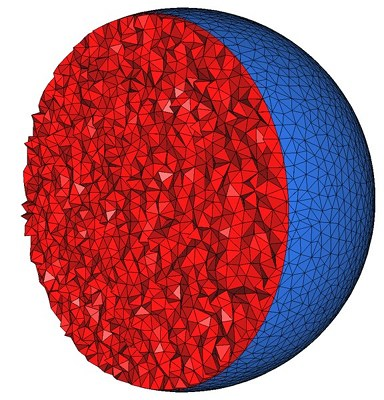
\includegraphics[width=\textwidth]{implicit_domain.jpg}
% % \end{center}
% % \end{column}
% % \end{columns}
% % \end{frame}
%
\section{Tests}

\begin{frame}[fragile]{Testing con Asserts en C++}
En C++, se pueden hacer pruebas unitarias utilizando asserts. 

\begin{itemize}
\item Un assert es una macro que verifica una expresión y termina el programa si la expresión es falsa.
\item Los asserts son útiles para detectar errores lógicos en el programa, como valores inválidos de parámetros o errores de cálculo.
\end{itemize}

Para utilizar los asserts, se debe incluir la biblioteca \texttt{cassert} y luego utilizar la macro \texttt{assert} con la expresión a evaluar:

\begin{minted}{c++}
#include <cassert>

int dividir(int a, int b) {
    assert(b != 0);
    return a / b;
}
\end{minted}

Si la expresión \texttt{b != 0} es falsa, el programa terminará en ese punto y mostrará un mensaje de error.

\end{frame}
%
\begin{frame}[fragile]{Google Test}
Google Test es un framework de testing más sofisticado

\begin{itemize}
\item Diversos tipos de asserts
\item Permite el uso de clases para crear suites de tests
\item Similar a \texttt{jUnit} de Java o \texttt{mUnit} de Scala
\item Su uso no es obligatorio pero muy recomendado
\end{itemize}

Para usarlo en conjunto con CMake: \url{https://google.github.io/googletest/quickstart-cmake.html}

O puede ver el siguiente video: \url{https://youtu.be/pxJoVRfpRPE?si=hqbv1whpbNtKcrzl}

\end{frame}
% \section{Compilación}
%
% \begin{frame}[fragile]{Compilación}
%     \begin{minted}[label=makefile]{cpp}
% all: maximo complejo rectangulo assert_ex iteradores rectangulo_ex1 
% maximo:
% 	g++ maximo.cpp -o maximo
% complejo:
% 	g++ complejo.cpp -o complejo
% rectangulo:
% 	g++ rectangulo.cpp rectangulo.hpp -o rectangulo
% rectangulo_ex1:
% 	g++ rectangulo_ex1.cpp -o rectangulo_ex1
% assert_ex:
% 	g++ assert_ex.cpp -o assert_ex
% iteradores:
% 	g++ iteradores.cpp -o iteradores
% clean:
% 	rm -f maximo complejo rectangulo assert_ex1
%     \end{minted}
% \end{frame}
%
\begin{frame}[fragile]{Esqueleto}
CMake y Gtest serán explicado en más en profundidad en la próxima auxiliar

\begin{minted}[label=root]{cmake}
cmake_minimum_required(VERSION 3.20)

project(CPPokemon)

set(CMAKE_CXX_STANDARD 20)
set(CMAKE_CXX_STANDARD_REQUIRED True)
set(CMAKE_EXPORT_COMPILE_COMMANDS True)

include(CTest)
add_subdirectory(external)
add_subdirectory(src)
add_subdirectory(test)

\end{minted}
\end{frame}

\begin{frame}[fragile]{Esqueleto}
\begin{minted}[label=src]{cmake}

add_library(${PROJECT_NAME} STATIC movement.cpp pokemon.cpp)
target_include_directories(${PROJECT_NAME} PUBLIC ${PROJECT_SOURCE_DIR}/include)

add_executable(${PROJECT_NAME}Run main.cpp)
target_link_libraries(${PROJECT_NAME}Run PUBLIC ${PROJECT_NAME})

\end{minted}

\begin{minted}[label=extern]{cmake}
add_subdirectory(googletest)
\end{minted}
\end{frame}

\begin{frame}[fragile]{Esqueleto}
\begin{minted}[label=test]{cmake}
if(BUILD_TESTING)
  add_executable(tests test.cpp)
  target_link_libraries(tests PRIVATE GTest::gtest_main ${PROJECT_NAME})
  add_executable(${PROJECT_NAME}::tests ALIAS tests)

  include(GoogleTest)
  gtest_discover_tests(tests)
endif()
\end{minted}
Puede ver en detalle el proyecto en la rama \texttt{reference}
\end{frame}
\section{Bibliografía}

\begin{frame}{Bibliography}

Stroustrup, B. (2018). A Tour of C++, Second Edition.


\begin{center}
      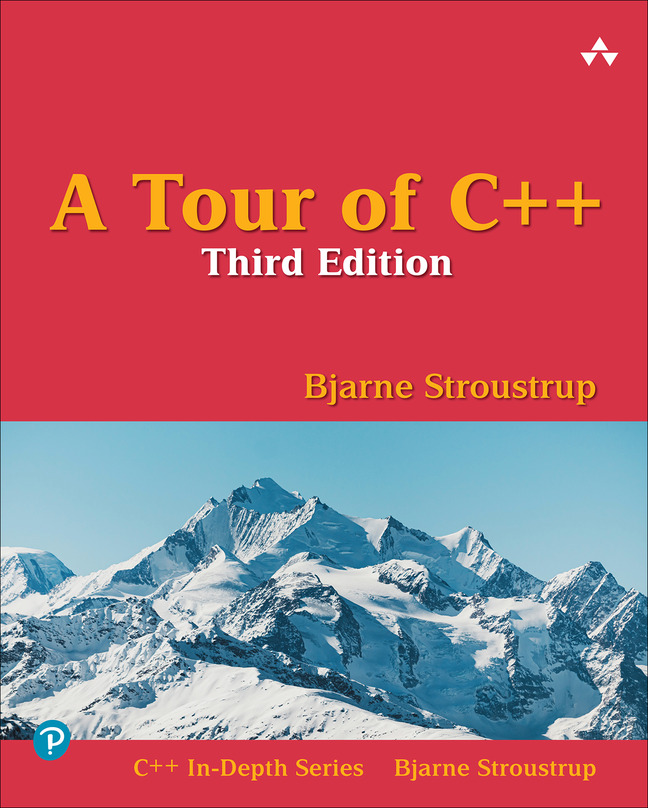
\includegraphics[height=8cm]{Tour3English-large.jpg}

\end{center}
    
\end{frame}

\end{document}
